\section{Einleitung}

Der Zeeman-Effekt beschreibt die Aufspaltung der Energieniveaus von Hüllenelektronen in einem Atom, die unter dem Einfluss eines Magnetfelds stehen. Dadurch ändern sich auch die Wellenlängen und Polarisationen, der ausgesandten Spektrallinien. Darüber kann der Effekt dann beobachtet und vermessen werden. Ziel dieses Versuchs ist es, den Zeeman-Effekt einer Cadmium-Lampe mithilfe eines Elektromagneten und einiger optischer Elemente aufzunehmen und die Aufspaltung zu vermessen.

\section{Theorie}
\label{sec:Theorie}

\subsection{Das magnetische Moment des Elektrons}

Die Hüllenelektronen eines Atoms besitzen aufgrund ihrer Ladung und ihren beiden Drehimpulsen, Bahndrehimpuls $l$ und Spin $s$, magnetische Momente.
Für die z-Komponente des magnetischen Moments gilt:
\begin{align}
  \mu_\text{Z} = -\frac{1}{2} \symup{e}_0 \frac{\hbar}{m_0} = \mu_\text{B}.\label{eqn:zKomp}
\end{align}
Dabei wird auch das Bohrsche Magneton $\mu_\text{B}$ definiert.
Nun setzen sich die Beträge des Bahndrehimpulses und des Spins aus den entsprechenden Quantenzahlen wie folgt zusammen:
\begin{align}
  |\vec l| &= \sqrt{l(l+1)}\hbar\\
  |\vec s| &= \sqrt{s(s+1)}\hbar.
\end{align}
Daraus folgt zusammen mit \eqref{eqn:zKomp} für die magnetischen Momente:
\begin{align}
  \vec\mu_l &= - \mu_\text{B} \frac{\vec l}{\hbar} = - \mu_\text{B} \sqrt{l(l+1)} \vec e_l\\
  \vec\mu_s &= - g_\text{S} \mu_\text{B} \frac{\vec s}{\hbar} = - g_\text{S} \mu_\text{B} \sqrt{s(s+1)} \vec e_s
\end{align}
Dabei ist $g_\text{S}$ der Landé-Faktor des Elektrons und beträgt ungefähr 2. Die Tatsache, dass das aus dem Spin folgende magnetische Moment etwa doppelt s groß ist, wie das aus dem Bahndrehimpuls folgende, wird als \textit{magnetomechanische Anomalie des Elektrons} bezeichnet.

\subsection{Wechselwirkung der Drehimpulse}

Die Wechselwirkung von Bahndrehimpuls und Spin ist im Allgemeinen sehr kompliziert und wird hier in zwei Grenzfällen beschreiben.

\begin{enumerate}
  \item Bei Atomen mit niedrigen Kernladungszahlen wechselwirken die Elektronen untereinander so stark, dass sich der gesamte Bahndrehimpuls der Hülle aus den Bahndrehimpulsen der einzelnen Elektronen zusammensetzt.
  \begin{align}
    \vec L = \sum \vec l_\text{i} \quad \text{mit} \quad |\vec L| = \sqrt{L(L+1)}\hbar
  \end{align}
  Abhängig von der Quantenzahl $L$ beschreibt man die Energieniveaus der Elektronen mit den Buchstaben S, P, D, und F. Wobei S für $L=0$, P für $L=1$ steht und so weiter. Der Gesamtspin $\vec S$ setzt sich in diesem Fall ebenfalls vektoriell zusammen und der Gesamtdrehimpuls ergibt sich dann aus der Addition aus Bahndrehimpuls und Spin durch die LS-Kopplung:
  \begin{align}
    \vec J = \vec L + \vec S
  \end{align}
  Die zum Gesamtdrehimpuls gehörende Quantenzahl $J$ wird als Index unten an die eben erwähnten Bahndrehimpulsbuchstaben geschrieben. Außerdem wird noch der Index $M$ oben an den Buchstaben geschrieben. Aus diesem kann über $M = 2S + 1$ die Spinquantenzahl $S$ entnommen werden. Diese Notation gilt für beide Fälle.
  \item Im Gegensatz zu der Drehimpulskopplung der Elektronen untereinander, koppeln bei schweren Atomen nur die beiden Drehimpulse der einzelnen Elektronen. So ergibt sich für jedes Elektron der Gesamtdrehimpuls nach:
  \begin{align}
    \vec j_\text{i} = \vec l_\text{i} + \vec s_\text{i}.
  \end{align}
  Der Gesamtdrehimpuls der Atomhülle eribt sich dann aus der vektoriellen Addition der einzelnen $\vec j_\text{i}$.
\end{enumerate}

Die Atome mit mittlerer Kernladungszahl wie auch das hier benutzte Cadmium befinden sich in dem fließenden Übergang zwischen diesen beiden Grenzfällen.
\subsection{Aufspaltung}

Das magnetische Moment des zuvor berechneten Gesamtdrehimpuls setzt sich vektoriell aus den einzelnen magnetischen Momenten $\vec\mu_\text{L}$ und $\vec\mu_\text{S}$ zusammen. Dabei ist der Betrag:
\begin{align}
  |\vec \mu_\text{J}| &= \mu_\text{B} g_\text{J} \sqrt{J(J+1)}\\
\intertext{mit dem Landé-Faktor}
  g_\text{J} &= \frac{3J(J+1)+S(S+1)-L(L+1)}{2J(J+1)}.\label{eqn:lande}
\end{align}
Wenn nun an das Atom und damit an die Elektronen der Hülle ein magnetisches Feld $\vec B$ angelegt wird, spalten die Energieniveaus der Elektronen auf. Dies folgt aus der Richtungsquantelung, einem Effekt aus der Quantenmechanik. Demnach sind zwischen magnetischen Moment $\vec \mu_\text{J}$ und dem äußeren Feld $\vec B$ nur Winkel möglich, bei denen
\begin{align}
  \mu_{\text{J}_\text{z}} = - m g_\text{J} \mu_\text{B}
\end{align}
gilt.
Dabei ist $m$ die Orientierungsquantenzahl, die in ganzzahligen Schritten von $-J$ bis $+J$ reicht. Daraus folgt auch, dass jedes Energieniveau in $2J+1$ Niveaus aufspaltet.

Es können nun über die Schrödingergleichung mithilfe einer längeren Herleitung gezeigt werden, dass für die Übergänge zwischen diesen aufgespalteten Niveaus Auswahlregeln existieren. Demnach sind nur solche Übergänge möglich, bei denen die Änderung von $m$ die Werte $0, -1$ oder $+1$ annimmt. Zudem ist eine Spektrallinie, bei der $\Delta m = 0$ ist, parallel zum $B$-Feld linear polarisiert. Wenn die Änderung der Orientierungsquantenzahl $\Delta m = ±1$ beträgt ist das ausgesandte Licht zirkular polarisiert um die Achse des $B$-Felds. Je nach Vorzeichen wechselt dabei die Drehrichtung der Polarisierung.

\subsection{Normaler und Anomaler Zeeman-Effekt}
\label{sec:normalanomal}
Je nachdem ob der Elektronenspin der Energieniveaus von Null verschieden ist oder nicht, spricht man von dem anomalen beziehungsweise von dem normalen Zeeman-Effekt.

\paragraph{Normaler Zeeman-Effekt:}
\label{sec:normalzee}

Der Name ist hier irreführend, wo doch der normale Zeeman-Effekt weitaus seltener auftritt. Bei diesem Fall ist $S=0$. Dadurch beträgt der Energieunterschied vom aufgespalteten Niveau zu dem Ausgangsniveau für alle $L$ und $J$:
\begin{align}
  \Delta E = \Delta m \mu_\text{B} B.
\end{align}
Da $m$ erneut die ganzzahlige Orientierungsquantenzahl ist, sind die Energieniveaus alle äquidistant. Wie sich die Niveaus unter dem normalen Zeeman-Effekt aufspalten und wie sich die drei Komponenten der abgestrahlten Spektrallinien aus den Übergängen ergeben ist in Abbildung \ref{fig:aufspaltung} zu sehen.
\begin{figure}
  \centering
  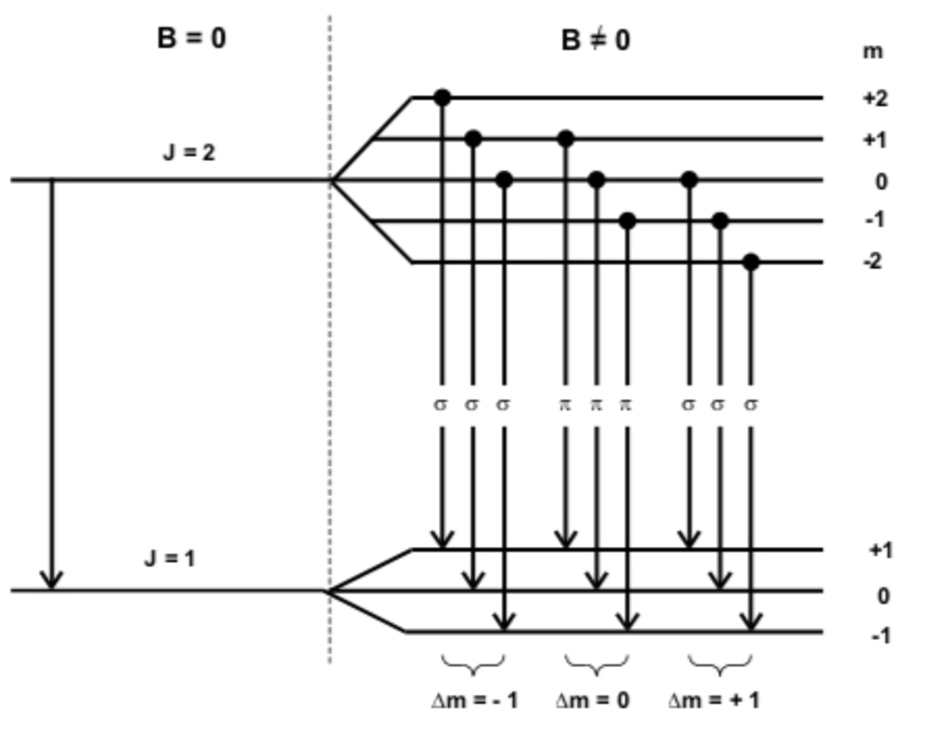
\includegraphics[height=9cm]{besuchInDerNacktmullAufzuchtstation/aufspaltung.pdf}
  \caption{Aufspaltung und Polarisation beim normalen Zeeman-Effekt \cite{anleitung}.}
  \label{fig:aufspaltung}
\end{figure}
Die $\pi$-Komponente ist dabei linear polarisiert. Beide $\sigma$-Komponenten sind in Feldrichtung zirkular polarisiert. Aus Gründen des leichteren Aufbaus werden hier alle Linien transversal zum Feld beobachtet. In dieser Richtung erscheinen auch die $\sigma$-Linien linear polarisiert, allerdings senkrecht zur $\pi$-Linie. Dadurch kann ein Polarisationsfilter die eine oder die andere Linie ausblenden.

Die rote Linie der Cadmium-Lampe an der der normale Zeeman-Effekt untersucht wird, entsteht bei einem Übergang von $^1P_1$ nach $^1D_2$. Demnach betragen die theoretischen Landé-Faktoren:
\begin{align}
  g_\text{J}(J=L=1, S=0) = \num{1.0} \quad g_\text{J}(J=L=2, S=0) = \num{1.0}.
\end{align}
Das entsprechende Termschema ist in Abbildung \ref{fig:normalTermschema}  zu sehen.
\begin{figure}
  \centering
  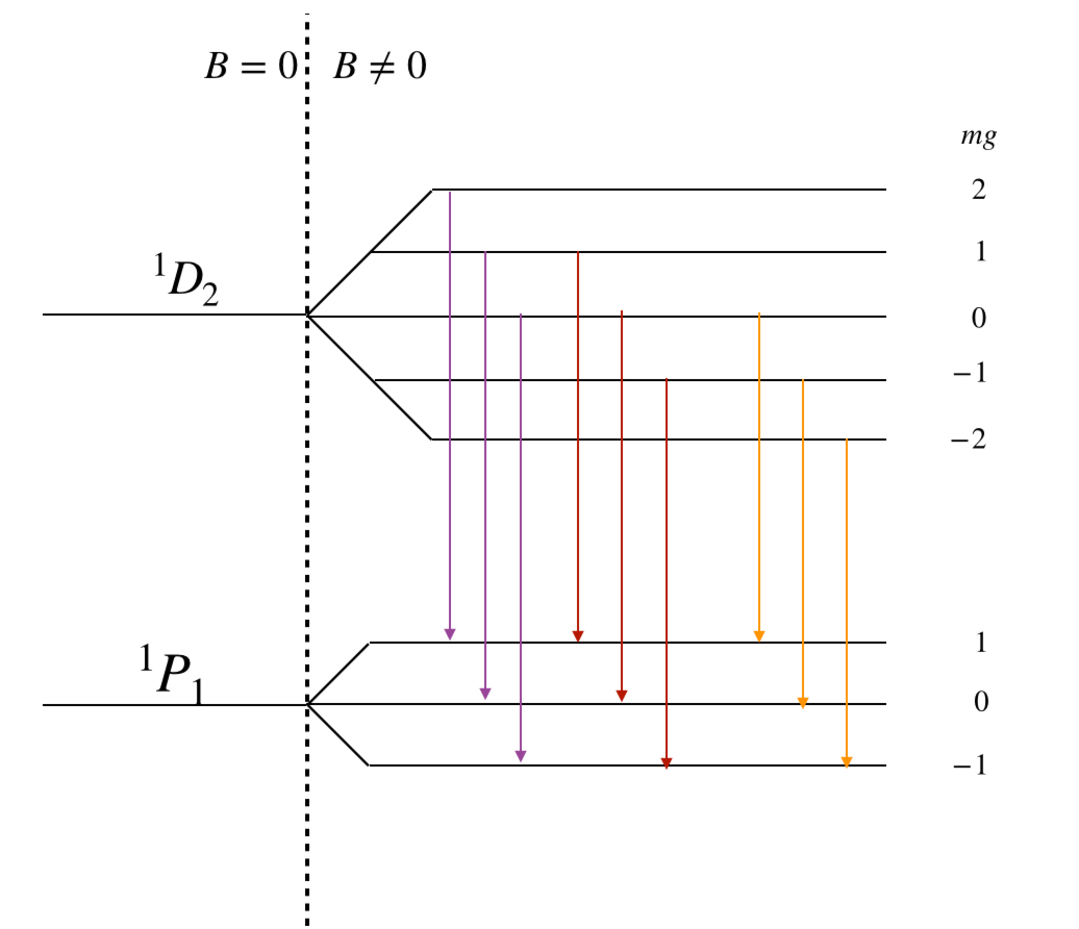
\includegraphics[height=10cm]{besuchInDerNacktmullAufzuchtstation/normalTermschema.pdf}
  \caption{Termschema des hier betrachteten normalen Zeeman-Effekts. Dabei sind die sechs äußeren Linien die $\sigma$-Komponenten mit $\Delta (mg) = \pm 1$ und die drei inneren Linien zählen zur $\pi$-Komponente mit $\Delta (mg) =  0$.}
  \label{fig:normalTermschema}
\end{figure}


\paragraph{Anomaler Zeeman-Effekt:}

In diesem Fall spielt der Elektronenspin eine Rolle, da $S\neq 0$. Hier sind die aufgespalteten Linien nicht mehr äquidistant. Daraus folgt, dass mehr Übergänge eistieren, die von der Energiedifferenz her verschieden sind. Also werden auch mehr Spektrallinien gesehen.
\begin{figure}
  \centering
  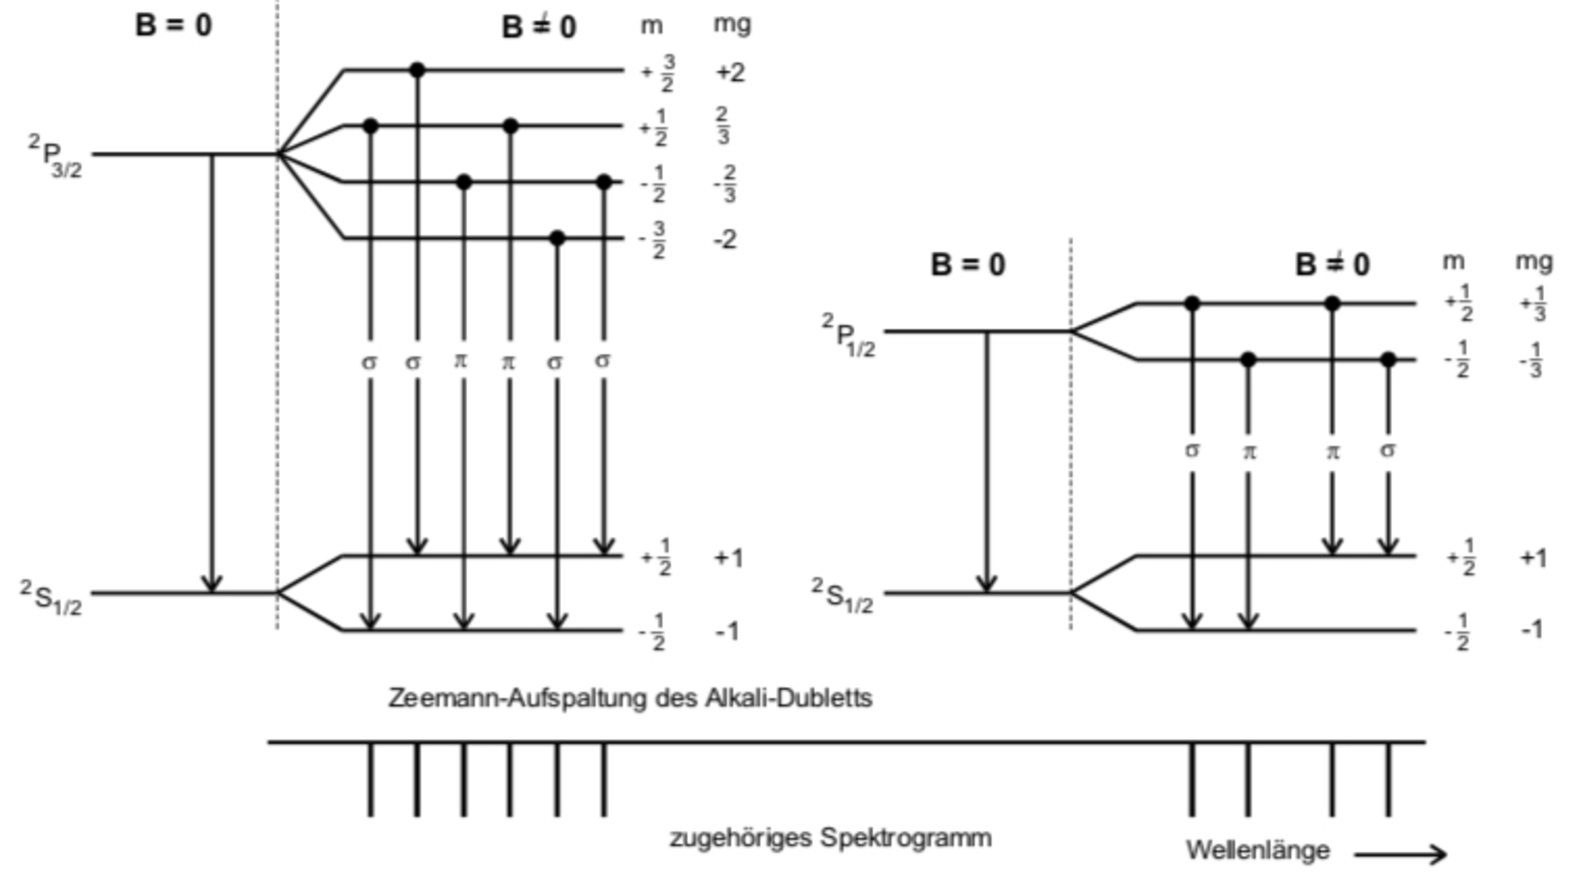
\includegraphics[height=10cm]{besuchInDerNacktmullAufzuchtstation/anomal.pdf}
  \caption{Aufspaltung und Polarisation beim anomalen Zeeman-Effekt \cite{anleitung}.}
  \label{fig:anomal}
\end{figure}
In Abbildung \ref{fig:anomal} ist an einem Beispiel gezeigt wie eine solche Aufspaltung aussieht.
Die Energiedifferenz der abgestrahlten Linie zur Linie bei $B = 0$ lässt sich dann durch
\begin{align}
  \Delta E = [m_1 g(L_1, S_1, J_1) - m_2 g(L_2, S_2, J_2)]\mu_\text{B} B\label{eqn:aufspaltungAnomal}
\end{align}
berechnen. Wobei sich der Landé-Faktor $g$ wieder aus Formel \eqref{eqn:lande} berechnet.

In diesem Fall wird der anomale Zeemaneffekt an der blauen Linie der Cadmiumlampe untersucht. Diese wird bei einem $^3S_1 \leftrightarrow ^3P_1$ Übergang transmittiert.
Hier ergeben sich für jedes Niveau eigene Landé-Faktoren. Das S-Niveau hat einen Faktor von:
\begin{align}
  g_\text{J}(L=0, J=1, S=1) = \num{2.0}
\intertext{und das P-Niveau einen von:}
  g_\text{J}(L=1, J=1, S=1) = \num{1.5}.
\end{align}
Das entsprechende Termschema ist in Abbildung \ref{fig:anomalTermschema}  zu sehen.
\begin{figure}
  \centering
  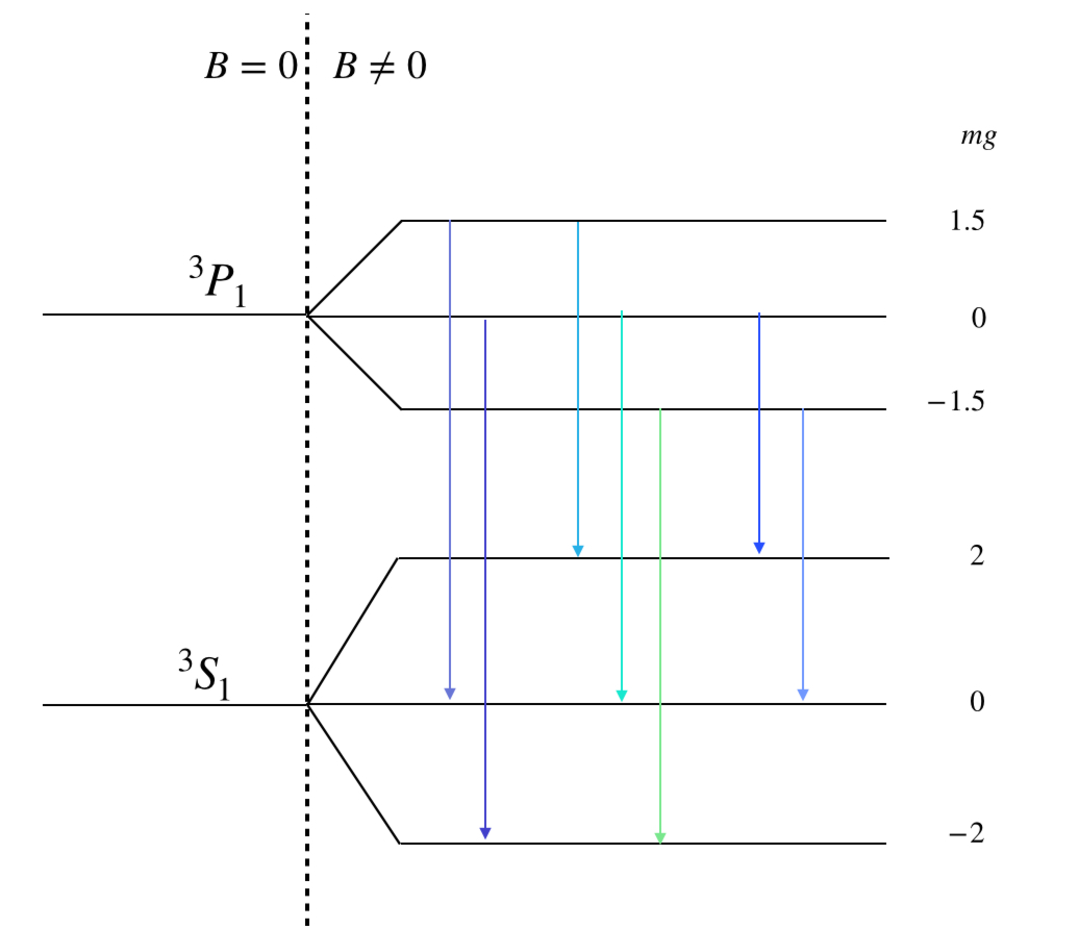
\includegraphics[height=10cm]{besuchInDerNacktmullAufzuchtstation/anomalTermschema.pdf}
  \caption{Termschema des hier betrachteten anomalen Zeeman-Effekts. Dabei sind die vier äußeren Linien die $\sigma$-Komponenten mit $\Delta (mg) = \pm [2; 1.5]$ und die drei inneren Linien zählen zur $\pi$-Komponente mit $\Delta (mg) =  [-0.5; 0; 0.5]$.}
  \label{fig:anomalTermschema}
\end{figure}


% \subsection{Fehlerrechnung}
%
% Für die Fehlerfortpflanzung bei Gleichungen mit $N$ fehlerbehafteten Größen
% wird jeweils die Formel zur Gaußschen Fehlerfortpflanzung
%
% \begin{equation*}
%   \sigma = \sqrt{\sum_{i=1}^{N}\biggl(\frac{\partial f(x_{\g{i}})}{\partial x_{\g{i}}}
%   \sigma_{\g{i}}\biggr)^2}
% \end{equation*}
% mit der jeweiligen Funktion $f(x_{\g{i}})$, den Messgrößen $x_{\g{i}}$ und den
% zugehörigen Fehlern $\sigma_i$ verwendet.
% Zur Berechnung des arithmetischen Mittels von $N$ Messwerten wird jeweils die
% Formel
%
% \begin{equation*}
%   \bar{x} = \frac{1}{N}\sum_{i=1}^{N}x_{\g{i}}
% \end{equation*}
% mit den Messwerten $x_i$ benutzt.
% Die Standardabweichung des Mittelwerts wird jeweils mit der Gleichung
%
% \begin{equation*}
%   \bar{\sigma} = \sqrt{\frac{1}{N-1}\sum_{i=1}^{N}(x_{\g{i}} - \bar{x})^2}
% \end{equation*}
% mit den $N$ Messwerten $x_i$ berechnet.


\cite{anleitung}
